\documentclass[11pt,a4paper]{article}
\author{TalentSprint}
\date{}
\usepackage{graphicx}
\usepackage{verbatim}
\usepackage{array}
\usepackage{caption}
\usepackage{enumitem}
\usepackage{xcolor}
\usepackage[tikz]{bclogo}
\usepackage{textcomp}
\usepackage{listings}
\usepackage{multicol}
\usepackage{float}
\usepackage{seqsplit} 
\usepackage{setspace}
\usepackage{soul}
\usepackage{latexsym}
\lstset{language=Java,numbers=left, numberstyle=\tiny, numbersep=10pt, showstringspaces=false, breaklines=true,keepspaces=true, columns=flexible}
\usepackage{fancyhdr}
\headheight=14pt
\lhead{\nouppercase{}}
\rhead{\nouppercase{\leftmark}}

\graphicspath{{../Images/}}


\begin{comment}
\setcounter{tocdepth}{1}
\setlength\parindent{0pt}
\parskip=4pt
\def\AnswerBox{\fbox{\begin{minipage}{4in}\hfill\vspace{0.5in}\end {minipage}}}

\thispagestyle{empty}
\vspace{1.5pc}
\topskip0pt
\vspace*{\fill}
\centerline{\sc \Huge Version Control System}
\vspace{2pc}
\vspace*{\fill}
\centerline{Prepared by TalentSprint WISE Team} 
\setcounter{page}{1}
\pagestyle{fancy}
\end{comment}


%========================================================================

% Lengths and widths
\addtolength{\textwidth}{2.5cm}
\addtolength{\hoffset}{0cm}
\setlength{\headsep}{-12pt} % Reduce space between header and content
\setlength{\headheight}{85pt} % If less, LaTeX automatically increases it
\renewcommand{\footrulewidth}{2pt} % Remove footer line
\renewcommand{\headrulewidth}{1pt} % Remove header line
\renewcommand{\seqinsert}{\ifmmode\allowbreak\else\-\fi} % Hyphens in seqsplit
% This two commands together give roughly
% the right line height in the tables
\renewcommand{\arraystretch}{1.3}
\onehalfspacing



% Commands
\newcommand{\SetRowColor}[1]{\noalign{\gdef\RowColorName{#1}}\rowcolor{\RowColorName}} % Shortcut for row colour
\newcommand{\mymulticolumn}[3]{\multicolumn{#1}{>{\columncolor{white}}#2}{#3}} % For coloured multi-cols
\newcolumntype{x}[1]{>{\raggedright}p{#1}} % New column types for ragged-right paragraph columns
\newcommand{\tn}{\tabularnewline} % Required as custom column type in use

% Font and Colours
\definecolor{HeadBackground}{HTML}{333333}
\definecolor{FootBackground}{HTML}{666666}
\definecolor{TextColor}{HTML}{333333}
\definecolor{DarkBackground}{HTML}{6B8E23} %{FD1AA8}
\definecolor{LightBackground}{HTML}{E8FED8} %D3FDC8
\definecolor{tit}{HTML}{FF6600}
\renewcommand{\familydefault}{\sfdefault}
\color{TextColor}
 \headsep = 25pt
% Header and Footer
\pagestyle{fancy}
\usepackage[headheight=110pt]{geometry}
\fancyhf{}% Clear header/footer

\fancyhead[r]{
\includegraphics[width = 4cm, height = 2cm]{TS-Logo.png}\hspace{0cm}}

%=================================TITLE=====================================
\fancyhead[l]{{\bf{\textcolor{tit}{\textrm{\large{Advanced Class Design}}}}}}
%===========================================================================

\renewcommand{\headrulewidth}{0.4pt}% Default \headrulewidth is 0.4pt
\renewcommand{\footrulewidth}{0.4pt}% Default \footrulewidth is 0pt

\rfoot{Page \thepage}
\lfoot{COPYRIGHT \textcopyright TALENTSPRINT, 2015. ALL RIGHTS RESERVED.}



\begin{document}

\section*{Packages and Import statements}

\subsection*{Packages}
A package is a namespace that organizes a set of related classes and interfaces. Conceptually you can think of packages as being similar to different folders on your computer.
\begin{description}
 \item Packages are important for three main reasons
 \begin{enumerate}
  \item They help in the overall organization of a project or library.
  \item Packages give you a name-scoping, to help to prevent collisions if many programmers in a company decide to make a class with the same name.
  \item Packages provide a level of security, because you can restrict the code, which you write so that only other classes in the same package can access it.
 \end{enumerate}

\end{description}

\subsubsection*{Creating a package}
\begin{itemize}
 \item Package statement should be the first non-comment line in the source code.
 \item Names of the package should be in lowercase.
 \item Package can have sub-package and are separated by a period separator (.)
 \begin{lstlisting}
 package com.pack;
 public class MyClass {
     // statement(s);
 }
\end{lstlisting}
 \item Compile the source file and execute as:
 \begin{figure}[H] 
 \begin{center}
  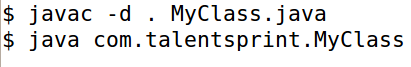
\includegraphics[scale=.5]{package.png}
 \end{center}
 \end{figure}
 
 \item A class must be in a directory structure that exactly matches the package structure. For a class, \emph{com.talentsprint.MyClass}, the \emph{MyClass} class must be in a directory named \emph{talentsprint}, which is in a directory named \emph{com}.
\end{itemize}

\vfill{\ }
\begin{figure}[H]
 \begin{center}
   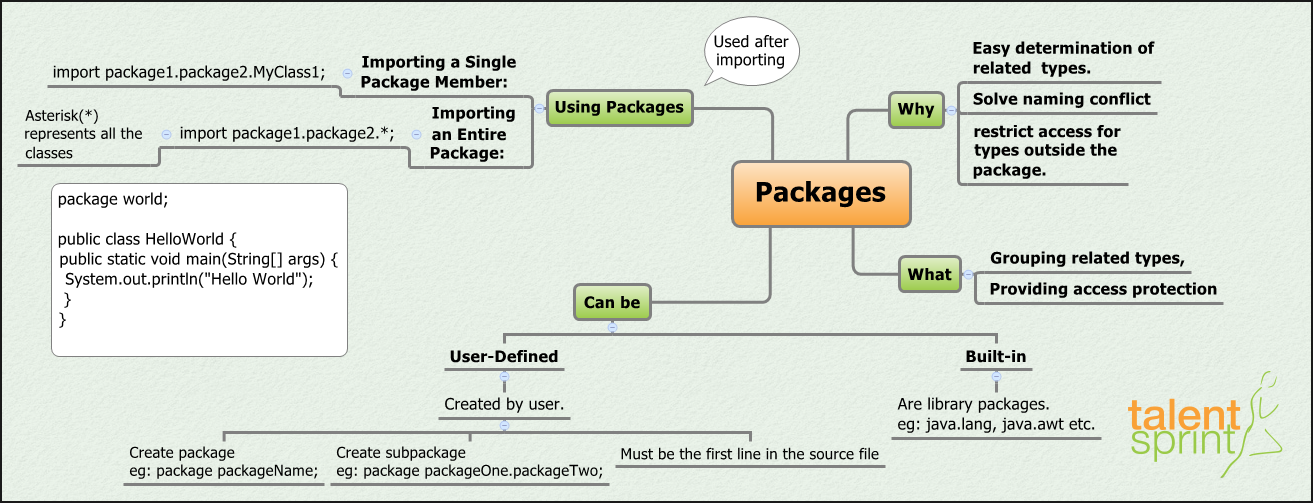
\includegraphics[angle=90,height=20cm, width=13cm]{Package-MM.png}
  
 \end{center}
 \end{figure}
 \subsection*{Import Statement}
 The import statements must come right after the package statement, before the class statement.
 \subsubsection*{Purpose of import statement}
  \begin{itemize}
   \item The rigid source code naming convention, the Java compiler can easily find the corresponding source or class files just from the fully qualified name of a package and class.
\begin{lstlisting}
import java.util.ArrayList;
public class MyClass {
    public static void main (String[] args) {
        ArrayList myList = new ArrayList(50);
        // Statement(s);
    }
}
\end{lstlisting}
\item If a class wants to use another class in the same package, the package name does not need to be used. Classes in the same package can find each other without any special syntax.  
\end{itemize}

\section*{Access Modifiers}
\emph{\textbf{Access modifiers}} defines the scope of a variable or method or class. There are four different types of access modifiers in Java:
\begin{enumerate}
 \item public (Least restrictive)
 \item protected
 \item default
 \item private (Most restrictive)
\end{enumerate}

\begin{description}
 \item [Public] specifies that class members (variables or methods) are accessible to anyone, both inside and outside of the class or package. Any object that interacts with the class can have access to the public members of the class
 \item [Protected] specifies that the class members are accessible only to methods in that class and the subclasses of the class. The subclass can be in different packages.
 \item [Default] specifies that only classes in the same package can have access to the variables and methods of the class. No actual keyword is used for the default modifier and it is applied in the absence of an access modifier.
 \item [Private] specifies that the class members are only accessible by the class in which they are defined.
\end{description}
Below is the sample code snippet that demonstrates how to use access specifiers
\begin{lstlisting}
 public class Student {
     public String name;  // public member
     protected int totalMarks; // protected member
     private double totalFeePaid; // private member
     int age; // default member
 }
\end{lstlisting}

\begin{description}
 \item Understanding from the above sample code snippet:
 \begin{description}
  \item [name] property/variable can access by any class member from anywhere.
  \item [totalMarks] property/variable can access by the class members itself and by its derived class members.
  \item [totalFeePaid] property/variable can access by the class members where it is defined. No other class or class members can access.
  \item [age] property/variable can access by any class which resides in the same package the class is defined.
 \end{description}
\end{description}

\subsubsection*{Java Program Structure: The Access Modifiers}

\begin{tabular}{|l|l|l|l|l|} \hline
 \multicolumn{1}{|c|}{ }  & \multicolumn{1}{|c|}{\textbf{private}} & \multicolumn{1}{|c|}{\textbf{default}} & \multicolumn{1}{|c|}{\textbf{protected}} & \multicolumn{1}{|c|}{\textbf{public}} \\\hline
 Same class & yes & yes & yes & yes \\\hline
 Same package & &  yes & yes & yes \\\hline
 Different package (sub-class) & & & yes & yes \\\hline
 Different package (non sub-class) & & & & yes \\\hline 
\end{tabular}

\section*{Methods}
A Java \emph{\textbf{method}} is a collection of statements that are grouped together to perform an operation and are used to communicate with objects. When we invoke or call a method we are asking the object to carry out a task, thus can say methods implement the behaviour of objects.  Methods are simillar to the functions in \textbf{C} - language. Every method needs to have name, required input parameters, return type and  set its visibility (private, protected or public).

\subsection*{Defining method} 
A method is just a chunk of code that does a particular job. The method structure contains method header and method body. The header contains return type, if any, a method name to identify the method and parameter(s) to pass values to the method. The body contains statements to perform the job.

\begin{lstlisting}[numbers=none]
 <modifier> <returnType> <methodName> (<parametersList>) {
    statement(s);
 }
\end{lstlisting}
Here is an example for a method named `getTotalMarks' that takes 3 parameters of marks and return the total of the marks.
\begin{lstlisting}
 /** The snippet returns the total of 3 marks */
 public int getTotalMarks(int marks1, int marks2, int marks3) {
    return marks1 + marks2 + marks3; 
 }
\end{lstlisting}

\subsection*{Method Calling}

The process of method calling is simple. When a program invokes a method, the program control gets transferred to the called method. This called method then returns control to the caller in two conditions, when:

\begin{enumerate}
 \item return statement is executed.
 \item reaches to the end of the method.
\end{enumerate}
 \begin{figure}[H] 
 \begin{center}
  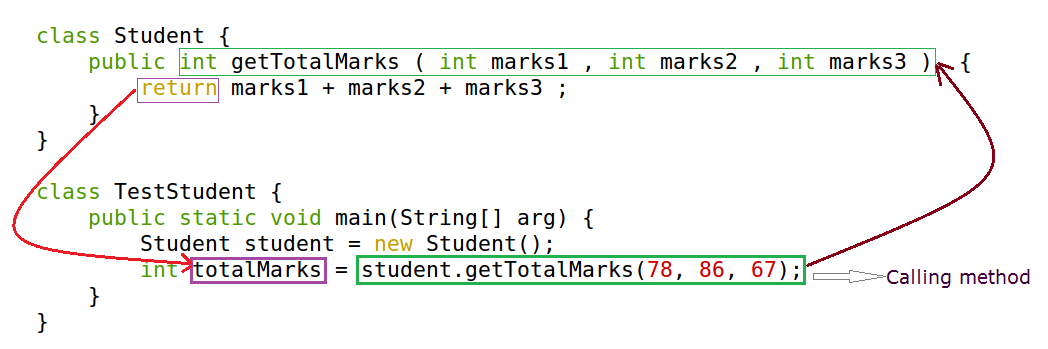
\includegraphics[scale=.45]{method-call.png}
\end{center}
 \end{figure}

\section*{Constructors}
%Java provides a special construct named constructor exclusively for creating an object of a class and initializing its instance variables.
Java constructors are the methods which are used to initialize objects. Constructors are called implicitly when an object is instantiated.

Keypoints to remember:
\begin{itemize}
 \item Constructor has the same name as the name of the class to which it belongs.
 \item Constructor is called or invoked when an object of class is created and can't be called explicitly.
 \item Constructor is generally declared as public.
 \item Constructor may have optional list of arguments.
 \item Constructor does not have any return type and not even void, since constructors never return a value.
 \item Constructor cannot invoke on an existing object.
 \item Constructor is used only in combination with the \lstinline!new! operator, which is used to instantiate an object.

To declare a constructor, you write,
\begin{lstlisting}[numbers=none]
 <modifier> <className> (<parametersList>) {
    statement(s);
 }
\end{lstlisting}
\end{itemize}
Constructors are two types
 \begin{description}
  \item [Default Constructor] is a constructor that doesn't have any parameters. If the class does not specify any constructors, then an implicit default constructor is created
  \begin{description}
  \item [Syntax] for default constructor
  \begin{lstlisting}[numbers=none]
   class <ClassName> {
       <ClassName>() {
           // Statement(s);
       }
   }
  \end{lstlisting}
 \end{description}
 \item [Parameterized constructor] is a constructor that has parameters. These are required to pass parameters on creation of objects. Parameterized constructor is used to provide different values to the
distinct objects.
\begin{description}
  \item [Syntax] for parameterized constructor
  
   \begin{lstlisting}[numbers=none]
   class <ClassName> {
       <ClassName>(<parametersList>) {
           // Statement(s);
       }
   }
  \end{lstlisting}
  \end{description}
 \end{description}
 
\subsubsection*{Invoking Constructors}
Constructors are invoked while creating an object using \lstinline!new! operator.
\begin{lstlisting}
class Student {
    // Instance variables
    // Default constructor
    Student() {
        // Statement(s);
    }
    
    // Parameterized constructor
    Student(String name, String branch) {
        // Statement(s);
    }

    public static void main( String[] args ){
        //create objects for Student class
        // Invokes default constructor
        Student = new Student();
        // Invokes parameterized constructor
        Student studentCris = new Student(``Surya'', ``CSE'');
        //some code here
    }
}
\end{lstlisting}
\vfill{\ }
\begin{figure}[H]
 \begin{center}
   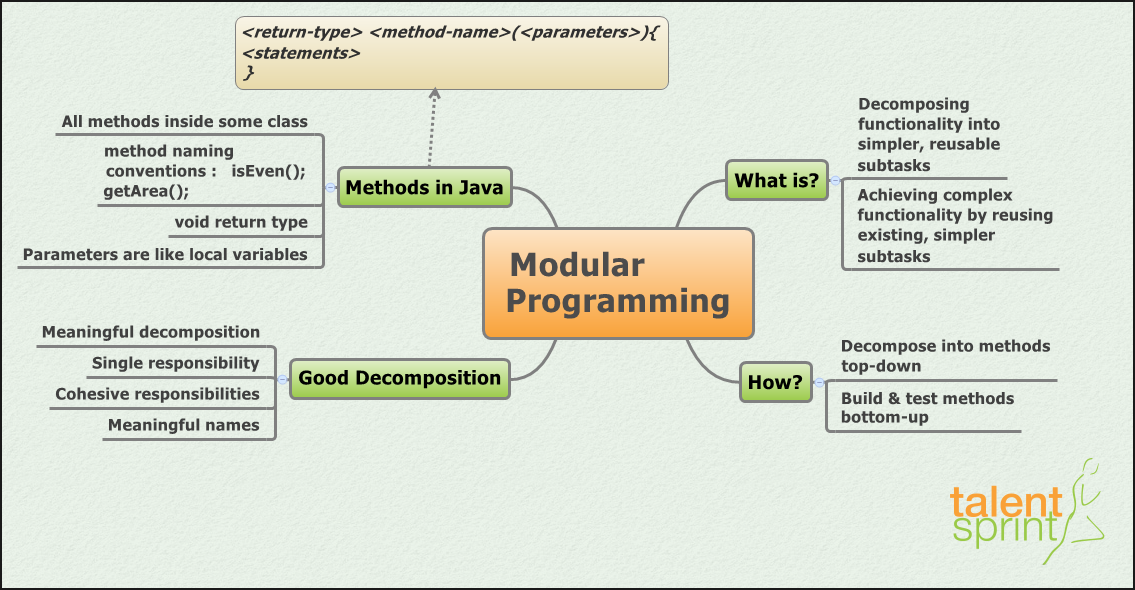
\includegraphics[angle=90,height=18cm, width=13cm]{ModularProgramming.png}
  
 \end{center}
 \end{figure}


\subsubsection*{this keyword}
 \emph{\textbf{this}}  is a keyword in Java. Which can be used inside method or constructor of  class. It works as a reference to current object whose method or constructor is being invoked.  \emph{\textbf{this}} keyword can be used to refer any member of current object from within an instance method or a constructor.

%Within an instance method or a constructor, \emph{\textbf{this}} is a reference to the \emph{current object} — the object whose method or constructor is being called.

\begin{description}
 \item [this] keyword with constructor (Constructor chaining)
 \begin{itemize}
  \item Constructor calls can be chained, which means that one constructor can call another constructor. \emph{\textbf{this()}} method is used for this purpose.
  \item There are a few things to remember when using \emph{this()} method in constructor call
  \begin{itemize}
   \item When using this in constructor call, it must occur as the first statement.
   \item It can only be used in a constructor definition. The this call can then be followed by any other relevant statements.
  \end{itemize}
  
  \begin{lstlisting}
class Student {
    public Student(){
        this("some string");
    }
    public Student(String str){
        // Statement(s);
    }
    public static void main( String[] args ) {
        Student student = new Student();
    }
}
  \end{lstlisting}

\end{itemize}
 \item[this] keyword with field (Instance Variable)
 \begin{itemize}
  \item \emph{\textbf{this}} keyword can be very useful in case of Variable Hiding.
  \item It(this) works as a reference to current object whose method or constructor is being invoked.
  \item To use this reference, you type, \lstinline!this.<Variable-Name >!
    
   \begin{figure}[H] 
 \begin{center}
 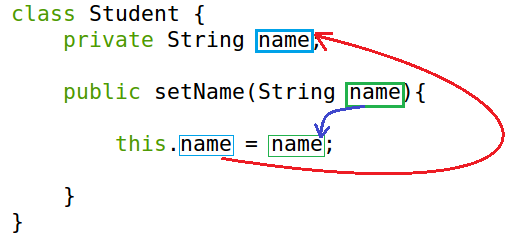
\includegraphics[scale=.7]{this-demo.png}
 \end{center}
 \end{figure}
 \end{itemize}
\end{description}

%===============================================================================================================================
\section*{Final keyword}
\lstinline!final! keyword in java is used to restrict the user. Final is a \emph{keyword} or \emph{reserved} word in java and can be applied to member variables, methods, class and local variables in Java. 
 Once you make a reference final you are not allowed to change that reference and compiler will verify this and raise compilation error if you try to re-initialized final variables in java.

\subsection*{Final classes}
A \lstinline!final! class cannot be subclassed or inherited. Several classes in Java are final. e.g. java.lang.String, java.lang.System, Integer and other wrapper classes.
 
Let us observe the following code snippet, where `Student' class is inherits a \lstinline!final! class `Person'
 \begin{lstlisting}[numbers=none]
 final class Person {
     // Instance variables
     // Instance methods
 }

 class Student  extends Person {  
     // Instance variables
     // Instance methods
 }
 \end{lstlisting}
 
 When you try to compile the above program, it display an compile time error, \emph{``cannot inherit from final class''}

\subsection*{Final Methods}
A \lstinline!final! method cannot be overridden or hidden by subclasses. This is used to prevent unexpected behavior from a subclass altering a method that may be crucial to the function or consistency of the class.


\begin{lstlisting}
class Person {
    public void eats() {
        // Statement(s);
    }
    public final void dateOfBirth() {
        // Statement(s);
    }
}
 
class Student extends Person {
     // Ok, overriding Person#eats()
    public void eats() {
        // Statement(s);
    }  
    
    // forbidden
    public void dateOfBirth() {    
        // Statement(s);
    }  
}
\end{lstlisting}

\subsection*{Final Variables}
A \lstinline!final! variable can only be initialized once, either via an initializer or an assignment statement. \lstinline!final! variable does not need to be initialized at the point of declaration: this is called a ``blank final'' variable. 
 \begin{itemize}
  \item A blank final instance variable of a class must be definitely assigned in every constructor of the class in which it is declared
  \item Similarly, a blank final static variable must be definitely assigned in a static initializer of the class in which it is declared
 \end{itemize}
 \begin{lstlisting}
class Student {
     
    public final String name;
    public final int age;
    public final String branch;
    Sphere(String n, int a, String b) {
         name = n;
         age = a;
         branch = b;
    }
    
    // Some methods
}
 \end{lstlisting}


\textbf{Benefits of final keyword in Java}
\begin{itemize}
 \item Final keyword improves performance. Not just JVM can cache final variable but also application can cache frequently use final variables.
 \item Final variables are safe to share in multi-threading environment without additional synchronization overhead.
 \item Final keyword allows JVM to optimize method, variable or class.
\end{itemize}
%=========================================================================
\section*{Static keyword}

  \lstinline!static! keyword in Java is used for memory management mainly. It can be applied to a field, a method or an inner class. A static field, method or class has a single instance for the whole class that defines it, even if there is no instance of this class in the program.

  \emph{\textbf{Note}}: For instance, a Java entry point (main()) has to be static.
   \begin{lstlisting}[numbers=none]
    public static void main(String args[])
 \end{lstlisting}

 \subsection*{static method}
 \lstinline!A static method cannot be abstract. It must be placed before the variable type or the method return type.!
 It is recommended to place it after the access modifier and before the final keyword. 
 
 Assume `getTotalMarks' method is final in `Student' class, then the method is defined as below code snippet
 
 \begin{lstlisting}
class Student {
    // Some variables and methods
    public static int getTotalMarks(Student []stArray) {
        double total = 0.0;
        //Statement(s);
        return total;
    }
}
 \end{lstlisting}
 
\lstinline!static! methods in Java can be called without creating an object of class.
 
\begin{lstlisting}
 class TestStudent {
     public static void main(String[] args) {
         int totalMarks = Student.getTotalMarks();
     }
 }
\end{lstlisting}

\subsubsection*{Keypoints to remember} 
 \begin{itemize}
  \item A static method belongs to the class rather than object of a class.
  \item A static method can be invoked without the need for creating an instance of a class.
  \item static method can access static data member and can change the value of it.
  \item The static method can not use non static data member or call non-static method directly.
  \item this and super cannot be used in static context.
  \end{itemize}
    
 \subsection*{static variables}
 A \lstinline!static! variable can be used as data sharing amongst objects of the same class. Mostly the \lstinline!static! variable is declared as \lstinline!public!. \lstinline!static! variables are common for each object of that class and there is only one instance of it. 
 %For example to implement a counter that stores the number of objects created at a given time can be defined as so:
 \begin{lstlisting}
 class Person {
     static String name;
 }
 \end{lstlisting} 

 \subsection*{static block} 
 A \lstinline!static! block is used to initialize the static data member and is executed before main method at the time of classloading.
\lstinputlisting{../Code/StaticBlock.java}
 Output
 \begin{figure}[H] 
 \begin{center}
  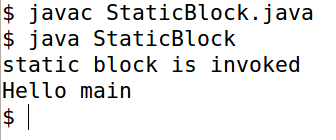
\includegraphics[scale=.5]{StaticBlock.png}
   
 \end{center}
 \end{figure}

%===============================================================================================================================
\section*{Garbage Collector}
Garbage collection is the systematic recovery of pooled computer storage that is being used by a program when that program no longer needs the storage. This frees the storage for use by other programs (or processes within a program).
Garbage collection is an automatic memory management feature in many modern programming languages, such as Java and languages in the .NET framework. Languages that use garbage collection are often interpreted or run within a virtual machine like the JVM. In each case, the environment that runs the code is also responsible for garbage collection.
Programs with an automatic garbage collector (GC) try to eliminate bugs by automatically detecting when a piece of data is no longer needed.

The Garbage Collector runs in a thread in the JVM. When the free memory drops under a threshold the GC begins to run to eliminate unneeded objects. Exactly when it runs and for how long, however, cannot be controlled by the user program.

\subsection*{Garbage-Collection Roots}
Every object tree must have one or more root objects. As long as the application can reach those roots, the whole tree is reachable. There are four kinds of GC roots in Java
\begin{enumerate}
 \item \textbf{Local variables} are kept alive by the stack of a thread. This is not a real object virtual reference and thus is not visible. For all intents and purposes, local variables are GC roots.
 \item \textbf{Active Java threads} are always considered live objects and are therefore GC roots. This is especially important for thread local variables.
 \item \textbf{Static variables} are referenced by their classes. This fact makes them de facto GC roots. Classes themselves can be garbage-collected, which would remove all referenced static variables. This is of special importance when we use application servers, OSGi containers or class loaders in general. We will discuss the related problems in the Problem Patterns section.
 \item \textbf{JNI References} are Java objects that the native code has created as part of a JNI call. Objects thus created are treated specially because the JVM does not know if it is being referenced by the native code or not. Such objects represent a very special form of GC root, which we will examine in more detail in the Problem Patterns section below.
  \begin{figure}[H]
 \begin{center}
   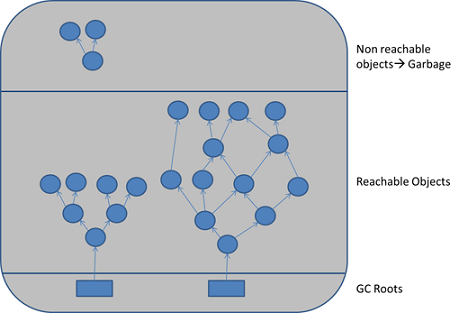
\includegraphics[scale=1.3]{gc.png}
 
 \end{center}
 \end{figure}
\end{enumerate}

\subsection*{Working with Garbage Collection}
Java garbage collection is an automatic process to manage the runtime memory used by programs. By doing it automatic JVM relieves the programmer of the overhead of assigning and freeing up memory resources in a program.

\subsubsection*{Garbage Collection GC Initiation}
Being an automatic process, programmers need not initiate the garbage collection process explicitly in the code. \lstinline! System.gc() and Runtime.gc()! are hooks to request the JVM to initiate the garbage collection process.
\subsubsection*{finalize() method}
Sometime an object will need to perform some specific task before it is destroyed such as closing an open connection or releasing any resources held. To handle such situation \lstinline!finalize()! method is used. \lstinline!finalize()! method is called by garbage collection thread before collecting object. Its the last chance for any object to perform cleanup utility.

The below code snippet shows how garbage collector is called explicitly using \lstinline!System.gc()!
\lstinputlisting{../Code/SystemGCDemo.java}

The below code snippet shows how garbage collector is called explicitly using \lstinline!Runtime.getRuntime().gc();!
%The program below shows that the garbage collection may run after \lstinline!System.gc()! is called. Again, it is NOT guaranteed.
\lstinputlisting{../Code/RuntimeGCTest.java}
The below code snippest shows that the garbage collection automatically works behind without \lstinline!System.gc()! called.
\lstinputlisting{../Code/GCTest.java}

\textbf{What does a GC perform?}
\begin{itemize}
 \item If a section of memory earlier used by an object is no longer referenced by any variable, then the Garbage Collector (GC) will release this memory for re-use by new objects. This takes place automatically without any input from the user program.
 \item There are no heap commands such malloc() and free() functions in C needed to allocate or de-allocate memory buffers.
 \item Java does use a similar ``new'' operator as in C++ for creating objects but has no ``delete'' operator.
\end{itemize}

\end{document}

